% !TeX root = 场论与凝聚态.tex
There might be a puzzle through the derivation above, 
\begin{quote}
    \emph{Before integrating out $\pi$, the $\exp$ term contains $\pi \mathrm{i} \partial_{\tau} \phi$. This match seems presentation-depending.
    How to figure out this mapping in a presentation independent way?}
\end{quote}


\subsection{General Development}
We' ve seen that a quantum field theory in $d+1$-dim spacetime can be reinterpreted as a $d$-dim space statistic field theory by regarding the time dimension as a inverse temperature, but it is not so obvious when we did not mop up the integration of conjugate momenta $\pi$. We need to find a way in whole, to figure out in what situation a quantum field theory can be seen as a statistic field theory. \emph{``Just as the time when we heard about the formalism of Lagrangian mechanic, all cumbersome processes of force analysis disappeared.''}

\textbf{The answer is by locality and unitarity.}

Let us first compare the behaviors between QFT and stat. mech.
\footnote{
    The properties mentioned in the table are only valid with an implicit assumption that the base manifold on which the field lives is orientable.
}
\begin{center}
    \begin{tabular}{|c|c|}
        \hline
        Real time & Imaginary time\\ 
        \hline & \\
        unitarity & reflection positivity\\ & \\
        \hline & \\
        \parbox{5cm}{\centering
            $\left( \mathrm{e}^{- \mathrm{i} H \Delta t} \right)^{*} = \mathrm{e}^{ - \mathrm{i} H (- \Delta t) }$
            \\
            $\Downarrow$
            \\
            $\mathop{\mathcal{Z}_{\mathbb{R} \times \Sigma}^{*} = \mathcal{Z}_{\mathop{\bar{\mathbb{R}}}\limits^{}_{\uparrow} \times \Sigma}}\limits^{}_{
                \hspace{5em} \text{orientation inversed}
                }
            $
            }&
        
        \parbox{5cm}{\centering
            also true because the only imaginary part is $\mathrm{e}^{- \int \mathrm{d} \tau \, \pi \mathrm{i}  \partial\tau \phi}$
            \\
            $\implies \mathcal{Z}^{*}_{\Sigma'} = \mathcal{Z}_{\bar{\Sigma}'}$
        } \\ & 

        \\ \hline

        \multicolumn{2}{|c|}{}\\

        \multicolumn{2}{|c|}{
            \parbox[h]{15cm}{The partition function of a locally defined theory can be splited into two parts, each on half of the base manifold. 
            For $\Sigma = \parbox[c]{2.8cm}{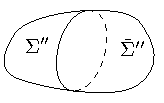
\includegraphics{figure_orientable_base.pdf}}$,
            the degree of freedom is the arbitrary boundary condition on $\partial \Sigma''$.
            By treating $\mathcal{Z}_{\Sigma''}$ and $\mathcal{Z}_{\bar{\Sigma}''}$ as functionals of $\left. \phi \right|_{\partial \Sigma''}$.
            we have 
            $$
            \mathcal{Z}_{\Sigma'} = \int  \left.\mathcal{D} \phi \right|_{\partial \Sigma''} \mathcal{Z}_{\Sigma''} \mathcal{Z}_{\bar{\Sigma}''} = \int  \left.\mathcal{D} \phi \right|_{\partial \Sigma''} \left( \mathcal{Z}_{\Sigma''} \right)  ^{2} \ge  0
            $$
            } 
        }\\
        \multicolumn{2}{|c|}{}\\
        \hline & \\

        \parbox{6cm}{\centering
            time reversal invariant \\
            $\Downarrow$ \\
            $\begin{cases} 
                \mathcal{Z}_{\Sigma' \times \bar{\mathbb{R}}} = \mathcal{Z}_{\Sigma' \times \mathbb{R}} \\
                \mathcal{Z}_{\Sigma'}^{*} = \mathcal{Z}_{\bar{\Sigma}'}
              \end{cases}
            $\\
            $\Downarrow$ \\
            $\mathcal{Z}$ is always real.
            }&
        \parbox{6cm}{
            \centering also \\ (useful in \emph{topological insulator})
            }
            \\ & \\
            \hline
        
    \end{tabular}
\end{center}
\clearpage
We have came to the conclusion that a theory with locality (of course with Hermitian Hamiltonian whilst) is always accompanied by a real and positive partition function $\mathcal{Z}$.


% might exist mistakes to be corrected

% In the following it will be convinced that \emph{if and only if} a Euclidean QFT admits \emph{Monte Carlo}, this QFT has a \emph{classical stat. mech. interpretation}.

% Sufficiency can be easily verified, as we have
% \begin{equation}
%   \mathcal{Z} = \int \mathcal{D} \phi  \, \exp\left( - \beta \int \mathrm{d} ^{d+1} r' \, \mathcal{H}(\phi) \right),
% \end{equation}
% where the integration of $\mathcal{D} \phi $ can be approximated by summation on a large amount of field configurations, which turns out to be Mont Carlo method. 

% Proof of necessity is carried out by utilizing locality
